\documentclass[a4paper,12pt]{article}

\usepackage[utf8]{inputenc}
\usepackage[T1]{fontenc}
\usepackage{a4}
\usepackage{lipsum}
\usepackage{graphicx}
\usepackage{float}
\usepackage{listings}
\usepackage{color}
\usepackage{hyperref}
\usepackage{cite}
\usepackage{textgreek}
\usepackage{amsfonts}

\usepackage[margin=1in]{geometry}

\title{
  {\Huge \bf Power Systems Lab}\\
  \vspace{0.25in}

  {\bf Experiment 9}\\
  Laboratory Report
  \vspace{1in}
}
\author{
  \bf Syed Alisamar Husain, 17BEE012\\
  B.Tech Electrical Engg, 8th Semester
}

\begin{document}
  \begin{titlepage}
    \maketitle
    \vspace*{\fill}
    \begin{center}
      {\bfseries Department of Electrical Engineering} \\
      Jamia Millia Islamia, New Delhi
    \end{center}
    \thispagestyle{empty}
  \end{titlepage}
  
  \newpage
  \begin{center}
    \huge Experiment 9
    \vspace{0.5in}
  \end{center}

  \section{Objective}
  Design a surge arrestor used in transmission lines
  using Simulink.

  \section{Theoretical Background}
  {\bf A surge arrester is a device to protect electrical equipment from over-voltage 
  transients} caused by external (lightning) or internal (switching) events. 
  Also called a surge protection device (SPD) or transient voltage surge 
  suppressor (TVSS), this class of device is used to protect equipment in 
  power transmission and distribution systems.
  
  The energy criterion for various insulation material can be compared by 
  impulse ratio. A surge arrester should have a low impulse ratio, so that 
  a surge incident on the surge arrester may be bypassed to the ground 
  instead of passing through the apparatus.

  To protect a unit of equipment from transients occurring on an attached 
  conductor, a surge arrester is connected to the conductor just before it 
  enters the equipment. The surge arrester is also connected to ground and 
  functions by routing energy from an over-voltage transient to ground if 
  one occurs, while isolating the conductor from ground at normal operating 
  voltages. {\bf This is usually achieved through use of a varistor, 
  which has substantially different resistances at different voltages.}
  
    \subsection{Construction of Metal Oxide Surge Arrester}
    The zinc oxide is a semiconducting material of N-type. It is pulverised and finely grained. 
    More than ten doping materials are added in the form of fine powders of insulating oxides 
    such as Bismuth, Antimony Trioxide, Cobalt Oxide, Manganese Oxide, Chromium oxide. 
    The powder is treated with some processes, and the mixture is spray dried to obtain a dry powder.
    The dry powder is compressed into disc-shaped blocks. 
    The blocks are sintered to obtain a dense poly- crystalline ceramic.
    The metal oxide resistor disc is coated with a 
    conducting compound to protect the disc from undesirable environmental effect.

    \begin{figure}[H]
      \centering
      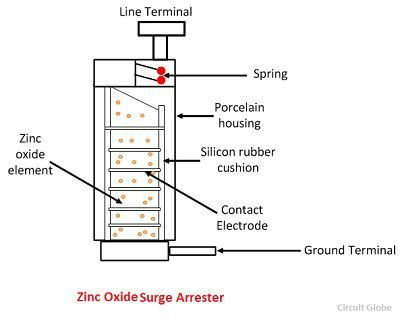
\includegraphics[width=3in]{img/ZNO-surge-diverter.jpg}
    \end{figure}

  \pagebreak
  \section{Implementation}
    \subsection{Basic Model}
    A basic Implementation can be done with a controlled current source triggered by a step
    function, via a parallel RL branch. The surge arrestors are between the line to ground.
    \begin{figure}[H]
      \centering
      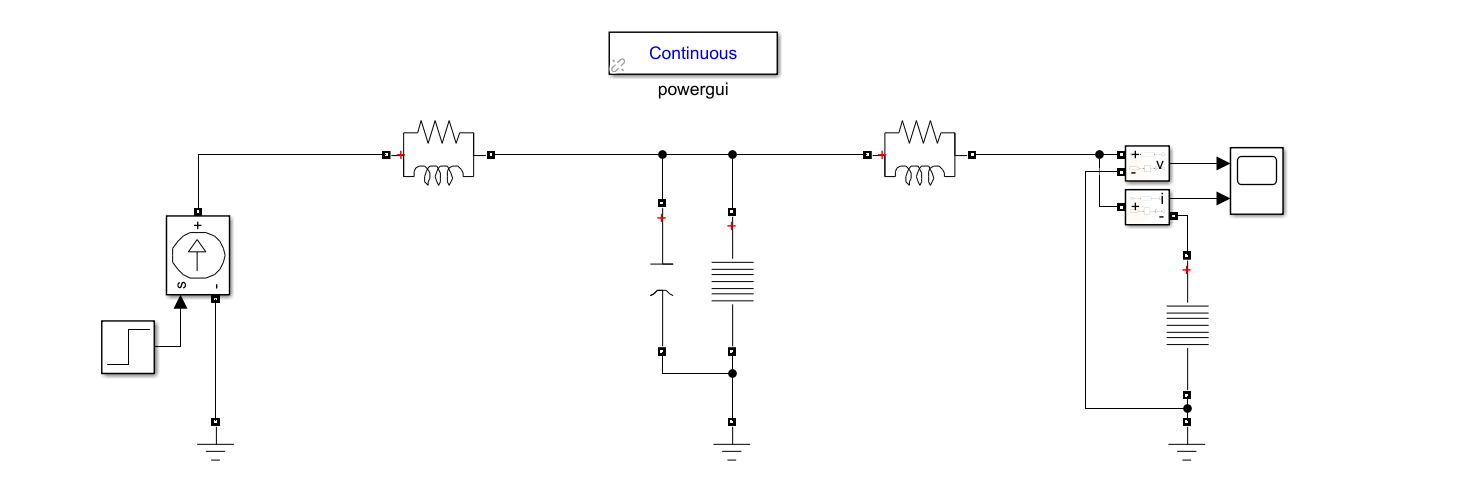
\includegraphics[width=6in]{img/basic.png}
    \end{figure}

    \subsection{Transmission Line Model}
    A 735 kV equivalent transmission systems feeds a load through a 200 km transmission line. 
    The line is series compensated at the middle point and shunt compensated at its receiving end. 
    {\bf A fault is applied at the load terminals.}

    The line is shunt compensated by a 110 MVAR per phase inductor at the load end.
    The line is protected by metal oxide varistors (MOV). The series varistor MOV1 consists 
    of 30 columns protecting the capacitor at 2.5 times its rated voltage 
    (rated voltage is obtained for a 2000 kA line rated current). 
    The corresponding protection voltage (defined at 500 A per column) is 185 kV.


    \begin{figure}[H]
      \centering
      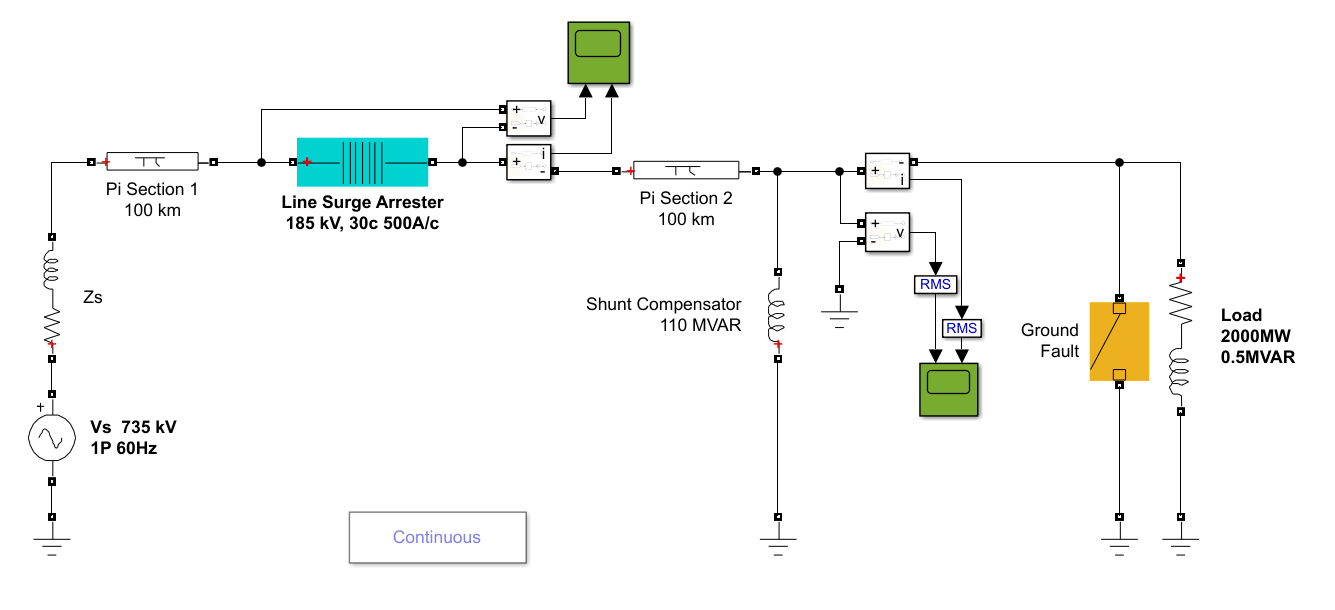
\includegraphics[width=6in]{img/model.png}
    \end{figure}

    For simplicity, only one phase of the transmission system is modeled. 
    All parameters correspond to positive-sequence.

  \pagebreak
  \section{Observations}  
  In the transmission line model, it is observed that at the moment of the fault, the load voltage
  should drop to zero but it doesn't since the surge arrestor continues to conduct.
  The load current peaks at 4900 A and stays constant during the fault.
  As the fault is cleared, both the load voltage and load current resume their initial values.
  \begin{figure}[H]
    \centering
    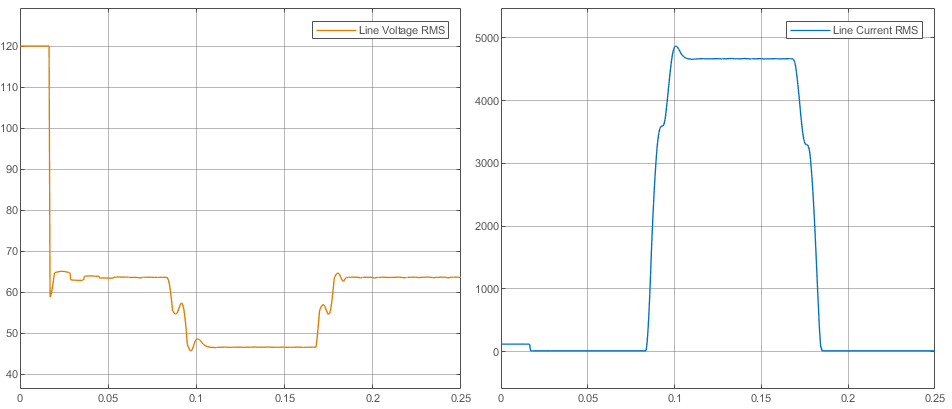
\includegraphics[width=6in]{img/line_current_rms.png}
    \caption{Load Voltage and Line Current (RMS)}
  \end{figure}

  \begin{figure}[H]
    \centering
    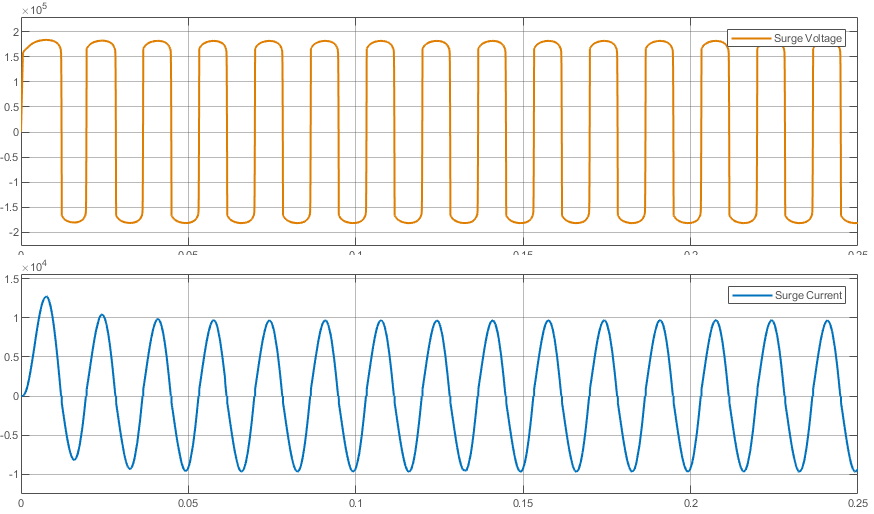
\includegraphics[width=5in]{img/line_surge.png}
    \caption{Voltage and Current through Surge Arrestor}
  \end{figure}

  \section{Result}
  We designed a model of a surge arrestor being used on a transmission line using Simulink,
  and observed the voltage and current charecteristics of the device during a fault condition.

\end{document}